% Options for packages loaded elsewhere
\PassOptionsToPackage{unicode}{hyperref}
\PassOptionsToPackage{hyphens}{url}
\PassOptionsToPackage{dvipsnames,svgnames,x11names}{xcolor}
%
\documentclass[
  11pt,
  letterpaper,
  DIV=11,
  numbers=noendperiod]{scrartcl}

\usepackage{amsmath,amssymb}
\usepackage{iftex}
\ifPDFTeX
  \usepackage[T1]{fontenc}
  \usepackage[utf8]{inputenc}
  \usepackage{textcomp} % provide euro and other symbols
\else % if luatex or xetex
  \usepackage{unicode-math}
  \defaultfontfeatures{Scale=MatchLowercase}
  \defaultfontfeatures[\rmfamily]{Ligatures=TeX,Scale=1}
\fi
\usepackage{lmodern}
\ifPDFTeX\else  
    % xetex/luatex font selection
\fi
% Use upquote if available, for straight quotes in verbatim environments
\IfFileExists{upquote.sty}{\usepackage{upquote}}{}
\IfFileExists{microtype.sty}{% use microtype if available
  \usepackage[]{microtype}
  \UseMicrotypeSet[protrusion]{basicmath} % disable protrusion for tt fonts
}{}
\makeatletter
\@ifundefined{KOMAClassName}{% if non-KOMA class
  \IfFileExists{parskip.sty}{%
    \usepackage{parskip}
  }{% else
    \setlength{\parindent}{0pt}
    \setlength{\parskip}{6pt plus 2pt minus 1pt}}
}{% if KOMA class
  \KOMAoptions{parskip=half}}
\makeatother
\usepackage{xcolor}
\setlength{\emergencystretch}{3em} % prevent overfull lines
\setcounter{secnumdepth}{5}
% Make \paragraph and \subparagraph free-standing
\ifx\paragraph\undefined\else
  \let\oldparagraph\paragraph
  \renewcommand{\paragraph}[1]{\oldparagraph{#1}\mbox{}}
\fi
\ifx\subparagraph\undefined\else
  \let\oldsubparagraph\subparagraph
  \renewcommand{\subparagraph}[1]{\oldsubparagraph{#1}\mbox{}}
\fi


\providecommand{\tightlist}{%
  \setlength{\itemsep}{0pt}\setlength{\parskip}{0pt}}\usepackage{longtable,booktabs,array}
\usepackage{calc} % for calculating minipage widths
% Correct order of tables after \paragraph or \subparagraph
\usepackage{etoolbox}
\makeatletter
\patchcmd\longtable{\par}{\if@noskipsec\mbox{}\fi\par}{}{}
\makeatother
% Allow footnotes in longtable head/foot
\IfFileExists{footnotehyper.sty}{\usepackage{footnotehyper}}{\usepackage{footnote}}
\makesavenoteenv{longtable}
\usepackage{graphicx}
\makeatletter
\def\maxwidth{\ifdim\Gin@nat@width>\linewidth\linewidth\else\Gin@nat@width\fi}
\def\maxheight{\ifdim\Gin@nat@height>\textheight\textheight\else\Gin@nat@height\fi}
\makeatother
% Scale images if necessary, so that they will not overflow the page
% margins by default, and it is still possible to overwrite the defaults
% using explicit options in \includegraphics[width, height, ...]{}
\setkeys{Gin}{width=\maxwidth,height=\maxheight,keepaspectratio}
% Set default figure placement to htbp
\makeatletter
\def\fps@figure{htbp}
\makeatother

% styles.tex
%\usepackage{cmbright}
\usepackage[dvipsnames]{xcolor}
\usepackage{sectsty}
\usepackage{titlesec}
\usepackage{tikz}
\usepackage{graphicx}

% Define red, centered Day headers
\titleformat{\section}
  {\normalfont\color{black}\centering\LARGE\bfseries}
  {\thesection}{1em}{}

\definecolor{flashcolor}{RGB}{221,217,195}


% Optional: Adjust subsection and subsubsection if desired
% \titleformat{\subsection}
%   {\normalfont\large\bfseries}{\thesubsection}{1em}{}
\KOMAoption{captions}{tableheading}
\makeatletter
\makeatother
\makeatletter
\makeatother
\makeatletter
\@ifpackageloaded{caption}{}{\usepackage{caption}}
\AtBeginDocument{%
\ifdefined\contentsname
  \renewcommand*\contentsname{Table of contents}
\else
  \newcommand\contentsname{Table of contents}
\fi
\ifdefined\listfigurename
  \renewcommand*\listfigurename{List of Figures}
\else
  \newcommand\listfigurename{List of Figures}
\fi
\ifdefined\listtablename
  \renewcommand*\listtablename{List of Tables}
\else
  \newcommand\listtablename{List of Tables}
\fi
\ifdefined\figurename
  \renewcommand*\figurename{Figure}
\else
  \newcommand\figurename{Figure}
\fi
\ifdefined\tablename
  \renewcommand*\tablename{Table}
\else
  \newcommand\tablename{Table}
\fi
}
\@ifpackageloaded{float}{}{\usepackage{float}}
\floatstyle{ruled}
\@ifundefined{c@chapter}{\newfloat{codelisting}{h}{lop}}{\newfloat{codelisting}{h}{lop}[chapter]}
\floatname{codelisting}{Listing}
\newcommand*\listoflistings{\listof{codelisting}{List of Listings}}
\makeatother
\makeatletter
\@ifpackageloaded{caption}{}{\usepackage{caption}}
\@ifpackageloaded{subcaption}{}{\usepackage{subcaption}}
\makeatother
\makeatletter
\@ifpackageloaded{tcolorbox}{}{\usepackage[skins,breakable]{tcolorbox}}
\makeatother
\makeatletter
\@ifundefined{shadecolor}{\definecolor{shadecolor}{rgb}{.97, .97, .97}}
\makeatother
\makeatletter
\makeatother
\makeatletter
\makeatother
\ifLuaTeX
  \usepackage{selnolig}  % disable illegal ligatures
\fi
\IfFileExists{bookmark.sty}{\usepackage{bookmark}}{\usepackage{hyperref}}
\IfFileExists{xurl.sty}{\usepackage{xurl}}{} % add URL line breaks if available
\urlstyle{same} % disable monospaced font for URLs
\hypersetup{
  colorlinks=true,
  linkcolor={blue},
  filecolor={Maroon},
  citecolor={Blue},
  urlcolor={Blue},
  pdfcreator={LaTeX via pandoc}}

\author{}
\date{}

\begin{document}
\begin{titlepage}
\centering


\includegraphics[width=0.8\textwidth]{UofGMS_header.png}

\vspace*{4cm}

\noindent\rule{\textwidth}{1pt}
{\Large \bfseries First GLE$^2$N workshop \par}

{\Huge \bfseries Translating Extreme Value Theory into Real-World Impact  \par}

{\large \bfseries XX October/December 2025 University of Glasgow, UK\par}

\noindent\rule{\textwidth}{1pt}
\vspace{1.5cm}

%{\fontsize{30}{28}\selectfont \bfseries Book of abstracts\par}
%\vspace{1.5cm}

%\includegraphics[width=0.3\textwidth]{hr_pic.png}

\begin{tikzpicture}[remember picture,overlay]
  \node[anchor=south west,inner sep=0pt]
       at ([xshift=30mm,yshift=10mm]current page.south west)
       {
\includegraphics[width=0.7\textwidth]{UofGMS_footer.png}};
\end{tikzpicture}

%\begin{tikzpicture}[remember picture,overlay]
%  \coordinate (anchor) at ([xshift=150mm,yshift=200mm]current page.south west);
%  \node[anchor=south west,inner sep=0pt] at (current page.south west)
%       {
\includegraphics[width=0.7\textwidth]{UofGMS_footer.png}};
%\end{tikzpicture}

%\begin{picture}(0,0)
%  \put(0,0){
\includegraphics[width=0.6\textwidth]{UofGMS_footer.png}}
%\end{picture}

\end{titlepage}
\clearpage
\setcounter{page}{1}

\ifdefined\Shaded\renewenvironment{Shaded}{\begin{tcolorbox}[boxrule=0pt, enhanced, borderline west={3pt}{0pt}{shadecolor}, interior hidden, sharp corners, frame hidden, breakable]}{\end{tcolorbox}}\fi

\renewcommand*\contentsname{Table of contents}
{
\hypersetup{linkcolor=}
\setcounter{tocdepth}{3}
\tableofcontents
}
\newcommand{\red}[1]{\textcolor{red}{#1}}

\newpage

\hypertarget{about-the-workshop}{%
\section{About the workshop}\label{about-the-workshop}}

\textcolor{red}{workshop theme needs to be defined}

This one-day workshop

\textbf{Goals}

\begin{itemize}
\item
  A
\item
  B
\end{itemize}

We hope that this collective effort will pave the way for \ldots{}

\newpage

\hypertarget{location-tbc}{%
\section{Location (TBC)}\label{location-tbc}}

We will meet in Seminar Room 311B, located on the third floor of the
Mathematics and Statistics Building
(\href{https://www.google.com/maps/place/School+of+Mathematics+and+Statistics/@55.8726073,-4.2944843,871m/data=!3m2!1e3!4b1!4m6!3m5!1s0x488845cfd066d839:0xeab86bed8f92f0d0!8m2!3d55.8726073!4d-4.2944843!16s\%2Fg\%2F11ddzkn8v0?entry=ttu\&g_ep=EgoyMDI1MDYwMS4wIKXMDSoASAFQAw\%3D\%3D}{Google
map}). The room is accessible by both stairs and lift. The building is
just a 6-minute walk from Hillhead subway station.

\begin{center}
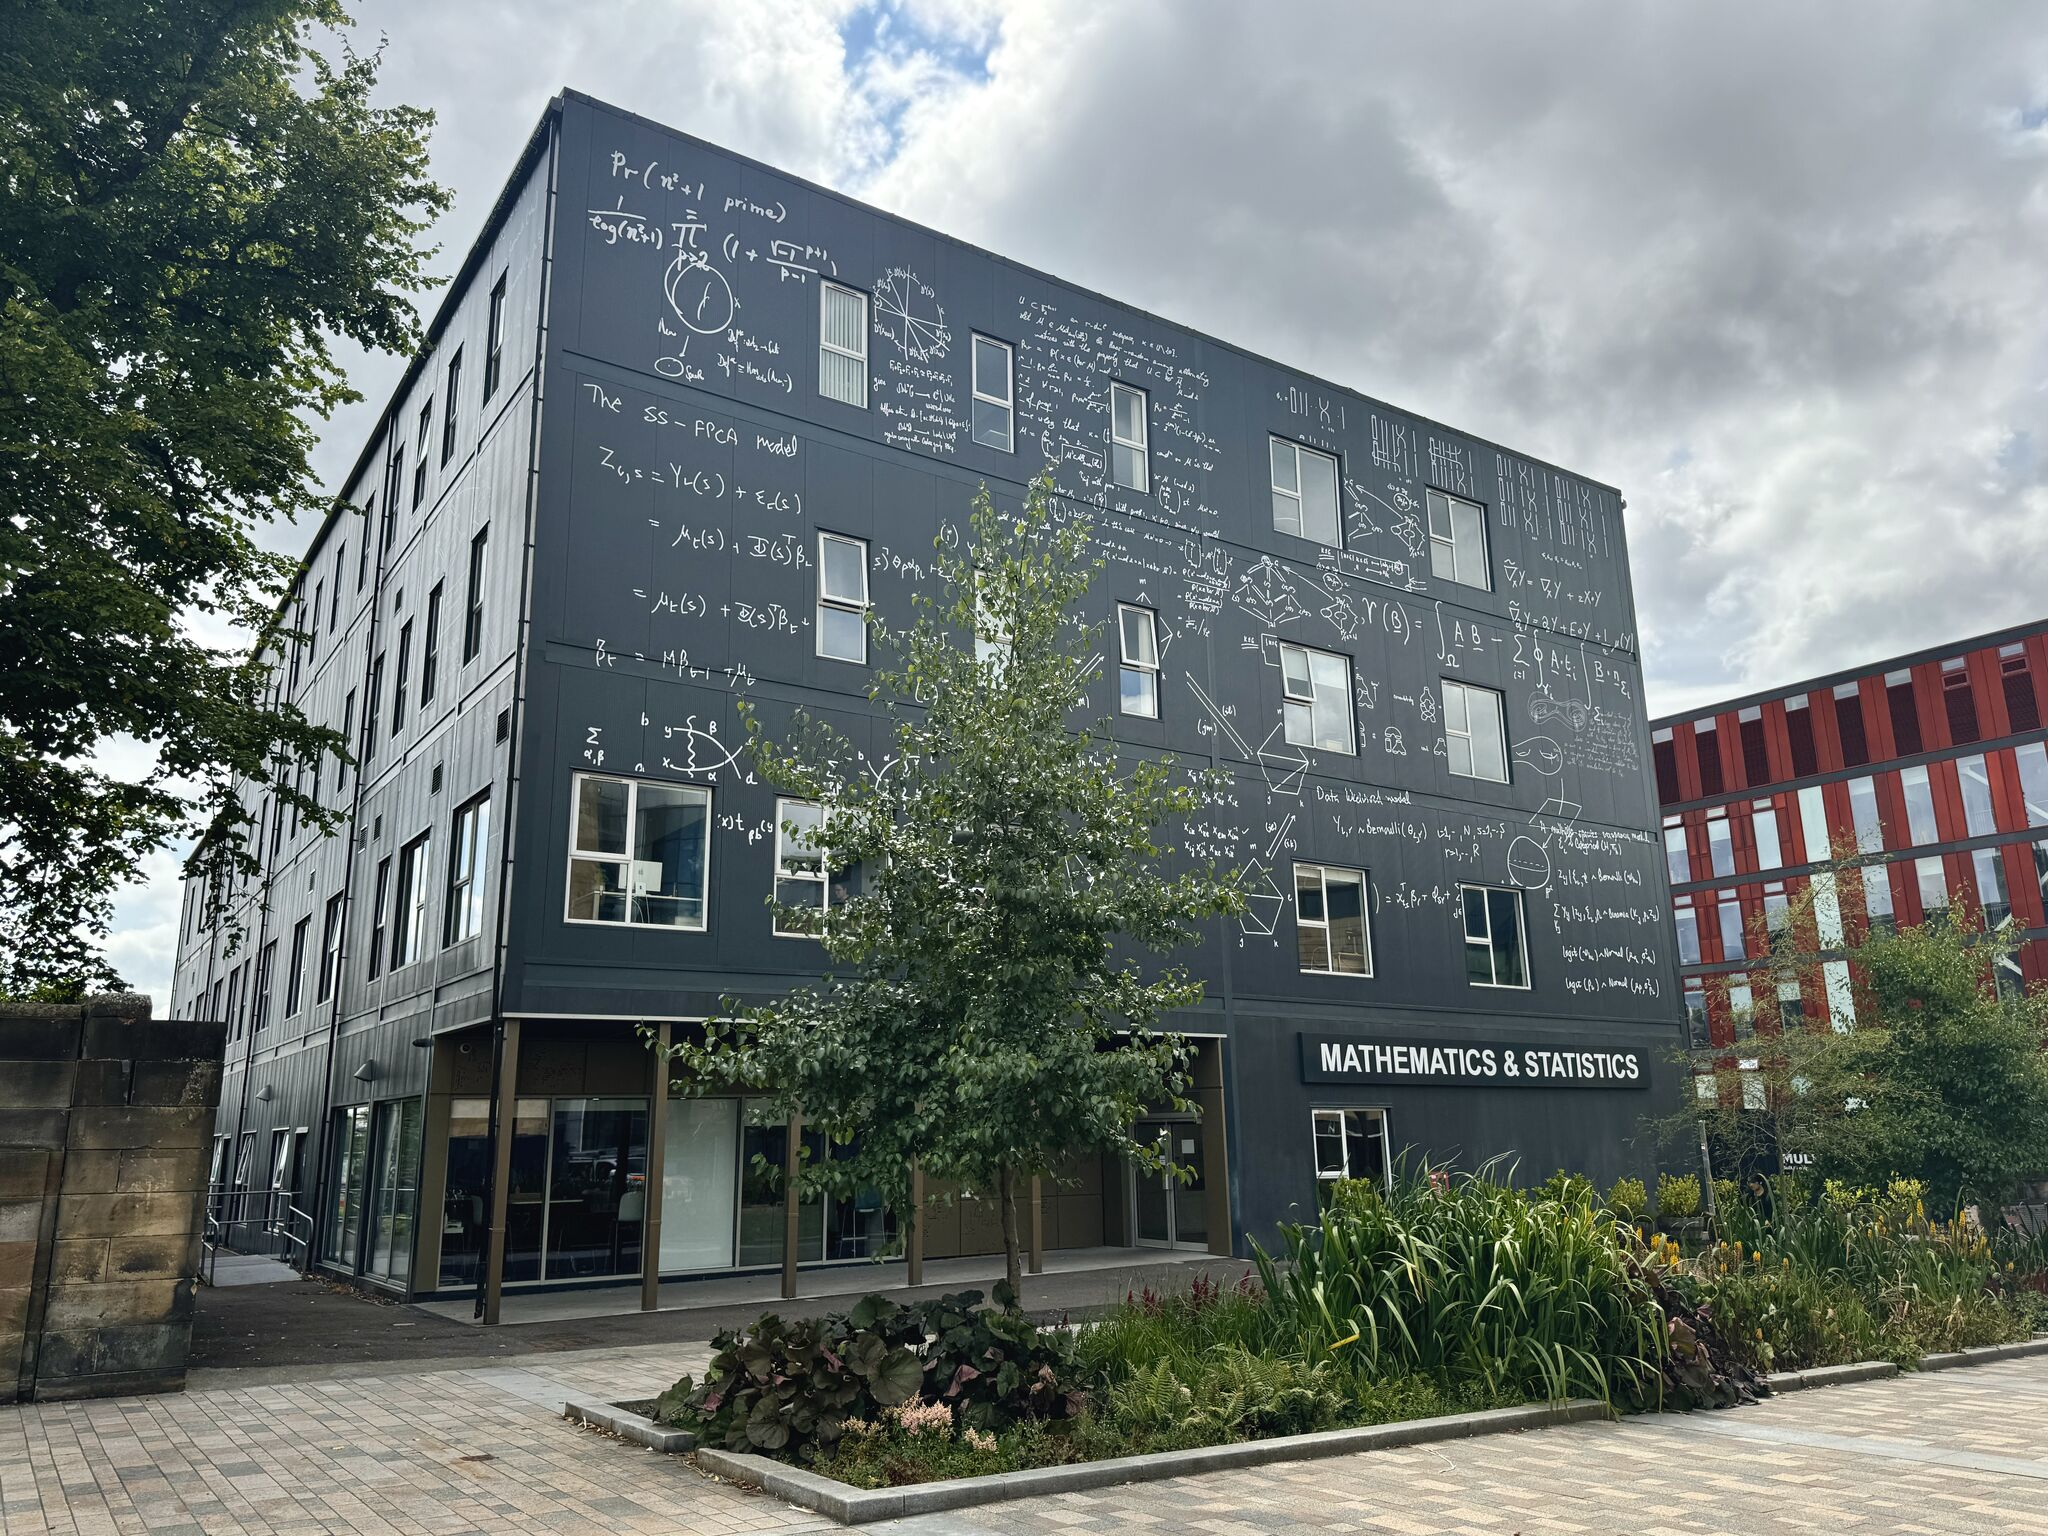
\includegraphics[width=0.6\linewidth]{ms-building.jpg}
\end{center}

\begin{center}
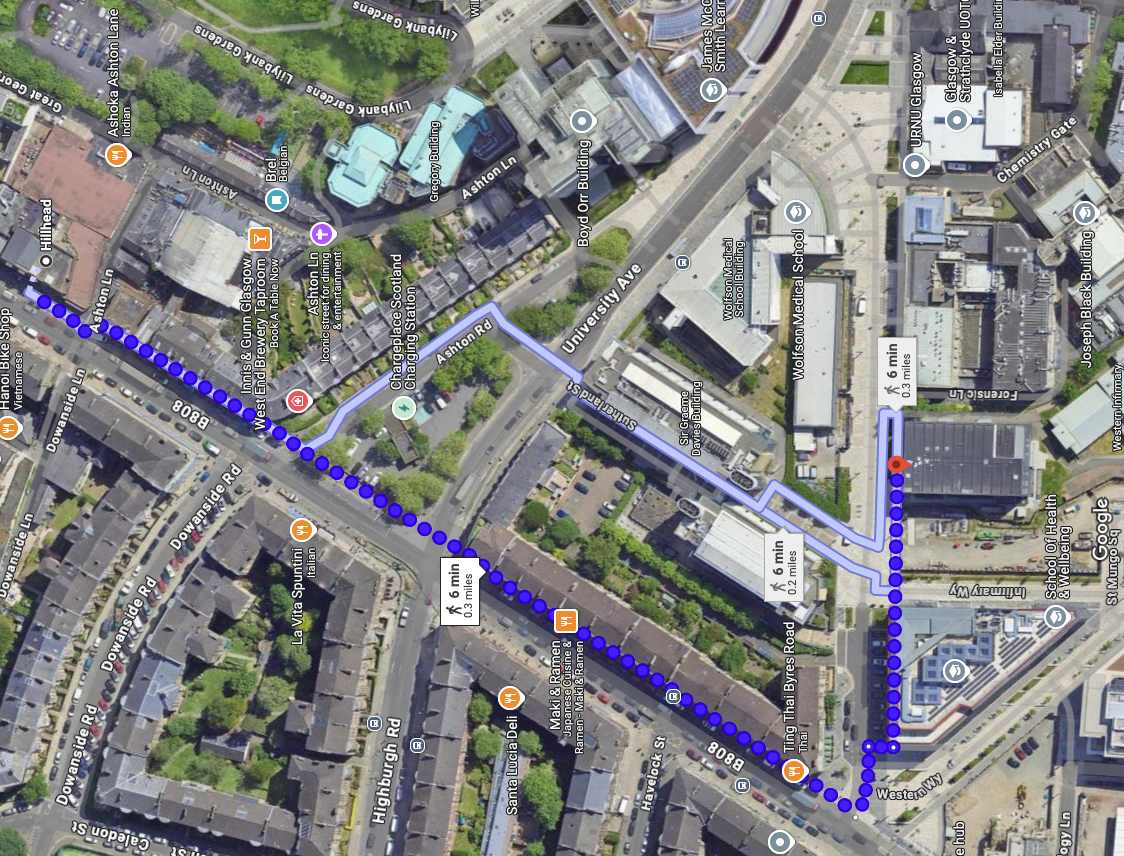
\includegraphics[width=0.6\linewidth]{map-to-ms.png}
\end{center}

\newpage

\hypertarget{programme-overview}{%
\section{Programme overview}\label{programme-overview}}

\textbf{9:15-9:30} --- Registration

\textbf{9:30-9:45} --- Welcome \& GLE²N presentation

\textbf{9:45-10:15} --- Optional 2-minute lightning intros (up to 15
attendees) \textcolor{red}{do we want to offer this to all?}

\textbf{10:15-10:45} --- Coffee break

\textbf{10:45-11:45} --- \textbf{Invited Talks Session 1} (2 × 25-minute
talks + 5 min Q\&A each)

\textbf{11:45-13:15} --- Lunch (not provided)

\textbf{13:15-14:15} --- \textbf{Invited Talks Session 2} (2 × 25-minute
talks + 5 min Q\&A each)

\textbf{14:15-15:15} --- \textbf{Contributed Talks} (4 × 12-minute talks
+ 3 min Q\&A each)

\textbf{15:15-15:45} --- Coffee break

\textbf{15:45-16:15} --- Discussion activity: theme review in teams

\textbf{16:15-16:45} --- Team reports \& group discussion

\textbf{16:45-17:00} --- Wrap-up \& closing remarks

\textbf{17:00 onwards} --- drinks \& dinner

\newpage

\hypertarget{abstracts}{%
\section{Abstracts}\label{abstracts}}

The grouping and sequence of talks aim to gradually build context---from
general frameworks and national challenges to specific methods and
applications---while maintaining variety and thematic coherence.

\newpage

\hypertarget{discussion-themes}{%
\subsection{Discussion Themes}\label{discussion-themes}}

Throughout the day, attendees are encouraged to contribute ideas,
questions, and provocations on the below themes using Post-it pads and
themed sheets placed around the room. These contributions will be used
in the afternoon discussion session.

\hypertarget{cross-disciplinary-collaboration}{%
\subsubsection{1. Cross-Disciplinary
Collaboration}\label{cross-disciplinary-collaboration}}

\emph{How can EVT more effectively contribute to interdisciplinary
challenges (e.g., climate, finance, health)?}

Prompt questions:

\begin{itemize}
\item
  What barriers exist when applying EVT in other scientific domains, and
  how can we lower them?
\item
  Are there successful case studies of EVT in interdisciplinary settings
  we can learn from?
\item
  How do we establish sustained collaborations with practitioners in
  fields like climate science, finance, or public health?
\end{itemize}

\hypertarget{scalability-computation}{%
\subsubsection{2. Scalability \&
Computation}\label{scalability-computation}}

\emph{What are the bottlenecks in applying EVT at scale, and how can we
overcome them (e.g., INLA, neural approaches)?}

Prompt questions:

\begin{itemize}
\item
  Which EVT models or inference techniques are most computationally
  efficient at scale?
\item
  What are the trade-offs between computational speed, model complexity,
  and interpretability?
\item
  How can we leverage modern computing tools (e.g., GPU,
  parallelisation, variational inference) to scale EVT methods?
\end{itemize}

\hypertarget{bridging-theory-and-practice}{%
\subsubsection{3. Bridging Theory and
Practice}\label{bridging-theory-and-practice}}

\emph{How do we translate advanced EVT theory into tools usable by
practitioners and stakeholders?}

Prompt questions:

\begin{itemize}
\item
  What makes a theoretical advance in EVT practically useful?
\item
  How can we communicate EVT model assumptions and uncertainties to
  non-specialists?
\item
  What types of user-friendly tools or software are most needed by
  practitioners?
\end{itemize}

\hypertarget{discussion-activity-details}{%
\subsection{Discussion Activity
Details}\label{discussion-activity-details}}

\hypertarget{task-1-theme-review-20-min}{%
\subsubsection{Task 1: Theme Review (20
min)}\label{task-1-theme-review-20-min}}

\begin{itemize}
\tightlist
\item
  Each group collects their theme sheet.
\item
  Review Post-it notes and prompt questions.
\item
  Summarise key ideas and explore potential answers or alternative
  approaches.
\end{itemize}

\hypertarget{task-2-team-reports-15-min-per-team}{%
\subsubsection{Task 2: Team Reports (15 min per
team)}\label{task-2-team-reports-15-min-per-team}}

\begin{itemize}
\tightlist
\item
  Each team leader presents their group's summary.
\item
  A short follow-up discussion with the full group.
\end{itemize}



\end{document}
